\subsection*{Úvod} 

Od začátku průmyslové revoluce, složitost výrobních strojů a sériových
linek se postupně narůstala a tim vyžadovala neustálé monitorování stavu
systémů, a to zejména z ekonomických důvodů.  Na druhou stranu systémy
vyžadujíci vysokou míru bezpečnosti jako letadla, kosmické lodě,
automobilové systémy, jaderné reaktory a další vyžadují okamžité spuštění
poplašného systému, lokalizování místa chyby a navíc možnost predikce
poruchy. Tyto požadavky se staly předpokladem pro vznik 
identifikace a detekce poruch a prediktivní údržby.

Výrobní proces vždy zahrnoval prvky kontroly chyb a online
monitorování. Od prvních metod detekce poruch, například vizuální
inspekce, dnešní továrny přecházejí na automatizované systémy skládající se
ze
senzorů a výpočetní techniky k vyhodnocení poruch.
Je potřeba monitorovat zařízení v reálném čase, aby nedošlo k poškození
způsobené chybou nebo anomálií. Každá jednotlivá chyba může zapřičinit zpomalení
výrobního procesu a tím i snížení zisku.

Algoritmy monitorování zařízení v reálném čase vytvořily Fault Detection
and Analysis (FDA). Metody FDA ve většině případech nevyžadují strojové
učení a dokáží detekovat poruchy pomocí základních algoritmů
jako Fourierova analýza a algoritmy pro kontrolu trendů apod.

Vzhledem k množství údajů nahromaděných v posledních letech a rozšíření
technologie ukládání dat jako cloudové služby a výpočetní efectivita, díky
nim je možné používat pokročilejší algoritmy pro detekci poruch a
analýzu. Pomocí technik klasifikace strojového učení je možné
lokalizovat místo chyby. Další možnosti, ktere jsou k dispozici za použití
velkého množství dat, je odhad zbývající doby použitelnosti (RUL) celého
systému. 

Tyto techniky vedly k prediktivni údržbé jakou je snaha optimálizací údržby.

Aktuální technický stav zařízení je vždy k dispozici podle informací
extrahovaných z měřených signálů. Je možné použít aktuální stav systému
pro odhad zbývající životnosti v jednotkach vzdálenosti nebo času. Odhadovaný zbytek
životností dává možnost plánování údržby vhledem ke skutečnému stavu systému.

Tyto algoritmy pro odhad životnosti, detekce poruch, techniky modelování a
identifikace systémů tvoří novou oblast prediktivní údržby.

Modelování systému umožňuje provádět experimenty a vyvíjet řešení
offline před fyzickou implementacemi v hardwaru. Nedostupné nebo
náročné  měření lze nahradit generovanými daty
ze simulačního modelu a nakonec simulační model pomáhá nasadit robustní
algoritmus.

Tato práce poskytuje krátký úvod do detekce poruch a predikce
metodiky údržby a základní terminologie.
Kapitola \ref{ch:teor_surv} popisuje hlavní cíl a problémy
v těchto oblastech, zaměřuje se na podobnosti a rozdíly mezi těmito 
dvěma přístupy.

Vývoj simulačního modelu dvojčinného pneumatického aktuátoru a
porovnání s reálným vybavením pomocí různých přístupů je
popsán v kapitolách 3, 4 a 5.

Následující kapitola 6 ilustruje prediktivní údržbu založenou na
signal-based
metodach využívajících různé senzory dostupné v demonstračním zařízení.
Aplikace předzpracování, extrakce features a trénování klasifikačního
modelu,
senzory byly hodnoceny z hlediska funkčnosti, přesnosti a ceny.

Model-based techniky prediktivní údržby založené vyuziti simulačního modelu
jsou popsány v kapitole 7. Pomocí simulační modelu lze
určit zbytkové signály mezi naměřenými daty a simulacímí daty z 
výstupu modelu. Pomocí simulačního modelu lze vygenerovávat údaje o degradaci
systemi a použit tyto data k odhadu zbývající životnosti.

\subsection*{Závěr}
Cílem této práce bylo představít a ověřit metody detekcí poruch a
techniky prediktivní údržby na dvojčinném pneumatickém pístu
jako objekt případové studie.

\subsubsection*{Simulační model}

Jedním z výstupů práce je simulační model
dvojčinného pneumatického pístového systému postaveného na základě diferenciálních rovnic
z pneumaticko-mechanické oblastí, modelováno a vyvíjeno pomocí
softwaru Matlab/Simulink. Parametry simulačního modelu byli odhadnuty v
nominalním stavu systému. Existuje však možnost
odhodou parametry poruchového stavu a simulovat systém při poruše.

Vzhledem k dostupným naměřeným údajům a výrazně nelineární dynamice
systému, simulační model vykazuje dobrou shodu s naměřeným
daty. Na rozdíl od modelu vytvořeného pomocí knihovny Simulink/Simscape je
výrazně méně výpočetně naročný při zachování numerické
stability. Tato fakta jsou zásadní, pro odhad parametrů.

Simulační model byl použit k experimentování s chováním systému za různých
podmínek, modelování poruchových situací a generování data pro design
a vyvoj robustních algoritmů prediktivní údržby.


\subsubsection{Signal-based PdM}
Dalším výstupem je ověření možnosti klasifikace a
detekce poruchového stavu pomocí technik prediktivní údržby,
na zakladé signal-based  metod. 

Pokusy byly prováděny na datové sadě měřené na demonstračním
zařízení pomocí osmi typů senzorů.
  
Signal-based metoda je založena na extrakci užitečných informací
přímo ze signálu v časově-frekvenčních doménách. Každý senzor vyžadoval
individuální přístup k předzpracování, extrahování features, hodnocení
vlastnosti a vytváření klasifikačních modelů. Ale obecně lze doporučit
minimální předběžné zpracování potřebné k uchování možných užitečných informací.

Tabulka \ref{tab:sensors_final} obsahuje srovnání senzorů ve dvou 
kategoriích, přesnost oveřená na testovacím datovém souboru a nákladéch.
Graf \ref{fig:sensors_final_bar} vizualizuje tyto údaje.

Překvapivě všechny senzory vykazovaly přesnost více než 75 \%. Mikrofony
nabízejí vynikající výkon z hlediska nákladů a přesnosti a jsou
vhodné pro instalaci a údržbu.

\begin{figure}[h!]
    \centering
    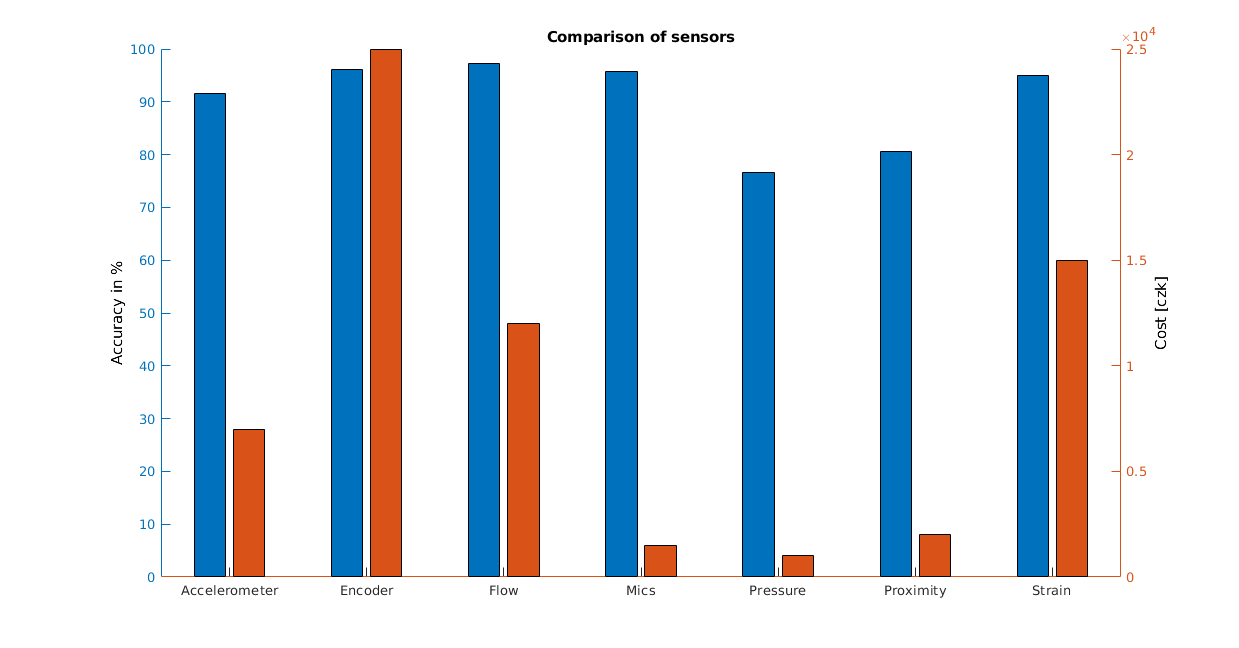
\includegraphics[width=1\textwidth]{sensors_final_bar.png}
    \caption{Comparison of sensors from accuracy/cost perspective}
    \label{fig:sensors_final_bar}
\end{figure}

\begin{table}[h]
    \centering
    \begin{tabular}{|c|c|c|c|c|c|c|c|}
        \hline
        \textbf{Sensor}   & Acc & Encoder & Flow & Mics & Pressure & Proximity & Strain \\
        \hline
        \textbf{Accuracy [\%]} & 91.6 & 96.1 & 97.2 & 95.8 & 76.6 & 80.5 & 95.0 \\
        \hline
        \textbf{Cost [czk]} & 2x 3500 & 25000 & 6000 & 3x 500 & 1000 & 2x 1000 & 15000 \\
        \hline
    \end{tabular}
    \caption{Comparison of sensors from accuracy/cost perspective}
    \label{tab:sensors_final}
\end{table}

\subsubsection*{PdM podle modelu}

Další částí této práce byla aplikace model-based metody a využití 
simulačního modelu pro algoritmy prediktivní údržby. Tyto algoritmy
jsou vhodné, pokud je těžké extrahovat užitečné informace přímo ze měřených
signálů. V některých případech, pokud rozumíme
dynamice systému, umíme využívat některé systémové proměnné jako
indikátory stavu.

Extrakce features ve formě nelineárních
koeficientu identifikačního modelu určeného z demonstračního zařízení,
konkrétně s Hammerstein-Wiener modelem, nedal spolehlivé výsledky.
Extrahované features nemají statistickou závislost a je nemožné předvídat typ poruchy
použitím této metody na naměřených datech z pneumatického pístu.

Na druhou stranu residual estimation methoda pomocí simulačního modelu
ukázala vynikající výsledky. Měřený signál polohy byl porovnán se
signálem ze nominalním simulačním modelem. Tento zbytkový
signál byl použit ke klasifikaci poruchového stavu a dosáhl 99 \% na
menší testovací datové sadě. Ale vzhledem k výsledkům získaným pomocí
signal-based metody, použití residual estimation se může zdát zbytečná. V
tomto konkrétním případé, z praktického hlediska, zlepšení
výsledeku o několik procent nepřináší zásadní změny, ale
doba výpočtu se významně zvyšuje.

Také byla ověřena možnost modelováni a simulace poruch senzorů
pomocí simulačního modelu. Ve většíně připadéch je náročné sbírat chybová
data způsobenými senzory vreálných podmínkách. Proto mohou být použity
generováne data ze simulačního modelu a pří kombinaci s původní
datovou sadou mohou vytvořit syntetický datový soubor.

\subsubsection*{RUL}

Jedním z hlavních cílů prediktivní údržby je odhadnout
zbývající životnost. Původní datová sada neobsahuje záznam o
historických datech, které ukazují degradační chování demonstračního
zařízení.

Běžným problémem při údržbě pneumatických pístů je netěsnost
vzduchu z komory, kde je umístěn píst. Tato situace byla
modelovaná na simulačním modelu a generovaná data byla použita pro RUL
odhad.

Vygenerovaná datová sada obsahuje 25 simulací s různou dynamikou poruch.
Každá simulace zahrnuje jiný počet cyklů v závislosti
na dynamice selhání. Každý cyklus
obsahuje 10-sekundové měření odezvy systému. V
experimentu byl jako předmět zájmu vybrán signál průtoku. Z
signálu průtoku, byl vypočítán parametr shape factor, který byl použit jako
indikátor stavu.

Výsledkem je možnost odhadnuti zbývající životnosti
na generovaném degradačním datovém souboru pomocí residual
similarity,  pairwise similarity a linear degradation modelu.
Předpovídané výsledky jsou uspokojivé (obr. \ref{fig:rul_deg_preforms}).

\begin{figure}[h!]
    \centering
    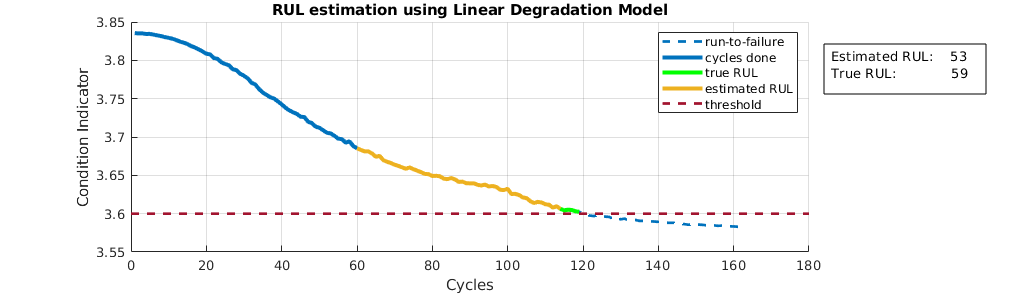
\includegraphics[width=1\textwidth]{rul_final.png}
    \caption{Linear degradation model performance}
    \label{fig:rul_deg_preforms}
\end{figure}


\subsubsection*{Další vývoj}

Pro další vývoj a zlepšení vysledků by bylo vhodné odhadnout
parametry systému po částech. S důrazem na
pracovní charakteristiku škrticích ventilů a tlumičů s příspůsobením.

Vhodným rozvojem by mohlo byt provedení měření poruchy úniku vzduchu a sběr
historické údaje o degradaci skutečného pneumatického pístu.
Následně vyhodnocení dynamiku poruchy způsobené únikem vzduchu,  
ověření možností odhadu zbývající životnosti pomocí snímače průtoku.

Mohla by to být zajímavá případová studie k ověření možnosti odhadu RUL
pomocí mikrofonů. Pokud jsou signaly z dostupných senzorů nedostačujicí
lze provádět měření tlaku v komoře. Tlak v
komoře je přímo závislý na úniku vzduchu z komory, jako
uvedené v rovnici \ref{eq:p_B_rul}. Příklad změn tlaku způsobených únikem vzduchu ze
simulačního modelu je znázorněn na obrázku \ref{fig:pressure_air_leak}.
